\section{Introduction}

\subsection{General steps to manufacture quantum dots}

The steps for manufacture are described below:\\

\begin{enumerate}[noitemsep]
\item Cleaving\\
    {\tiny 2.5mm x 5mm chip}
\item Cleaning\\
    {\tiny 5min hot NMP, 5min acetone, 5min IPA, 5min \SI{200}{\celsius} bake}
\item Resist spinning\\
    {\tiny Spin clean, AZ6612 (\SI{1.2}{\micro\meter})}
\item Photolithography (mesa pattern)
\item Resist developing\\
    {\tiny 55sec MIF300, 20sec DI \ce{H2O}}
\item Plasma Ash\\
    {\tiny 60 sec}
\item Mesa etching\\
    {\tiny 50sec etch soln (240/8/1 \ce{H2O}/\ce{H2O2}/\ce{H2SO4}), 20sec DI \ce{H2O} - \SI{2}{\nano\meter\per\second} etch rate}
\item Resist removal\\
    {\tiny 5min hot NMP, IPA}
\item Resist spinning\\
    {\tiny Spin clean, LOR20B (\SI{1.5}{\micro\meter}), AZ6612 (\SI{1.2}{\micro\meter})}
\item Photolithography (ohmics pattern)
\item Resist developing\\
    {\tiny 55sec MIF300, 20sec DI \ce{H2O}}
\item Plasma ash\\
    {\tiny 60 sec}
\item Metal deposition (ohmics)\\
    {\tiny \SI{50}{\angstrom} Ni, \SI{350}{\angstrom} Ge, \SI{720}{\angstrom} Au, \SI{180}{\angstrom} Ni, \SI{500}{\angstrom} Au}
\item Lift-off\\
    {\tiny 1Hr NMP}
\item Annealing\\
    {\tiny \SI{130}{\celsius} 1min (8s ramp), \SI{430}{\celsius} 2min (15s ramp)}
\item Resist spinning\\
    {\tiny Spin clean, PMMA A3}
\item Electron Beam Lithography (fine gates)
\item Plasma ash\\
    {\tiny 30 sec}
\item Metal deposition (fine gates)\\
    {\tiny \SI{80}{\angstrom} Ti, \SI{120}{\angstrom} Au}
\item Lift-off\\
    {\tiny 1Hr NMP, No sonication}
\item Imaging
\item Cleaning\\
    {\tiny 5min NMP, Acetone, IPA, no bake}
\item Resist spinning\\
    {\tiny LOR20B (\SI{1.5}{\micro\meter}), AZ6612 (\SI{1.2}{\micro\meter})}
\item Photolithography (large gates)
\item Resist developing\\
    {\tiny 55sec MIF300, 20sec DI \ce{H2O}}
\item Plasma ash\\
    {\tiny 60sec}
\item Metal deposition\\
    {\tiny \SI{120}{\angstrom} Ti, \SI{2000}{\angstrom} Au}
\item Lift-off\\
    {\tiny 1Hr NMP, No sonication}
\item Imaging
\end{enumerate}

\newpage

\subsection{Alignments DD V1}

\begin{figure} [h] \centering
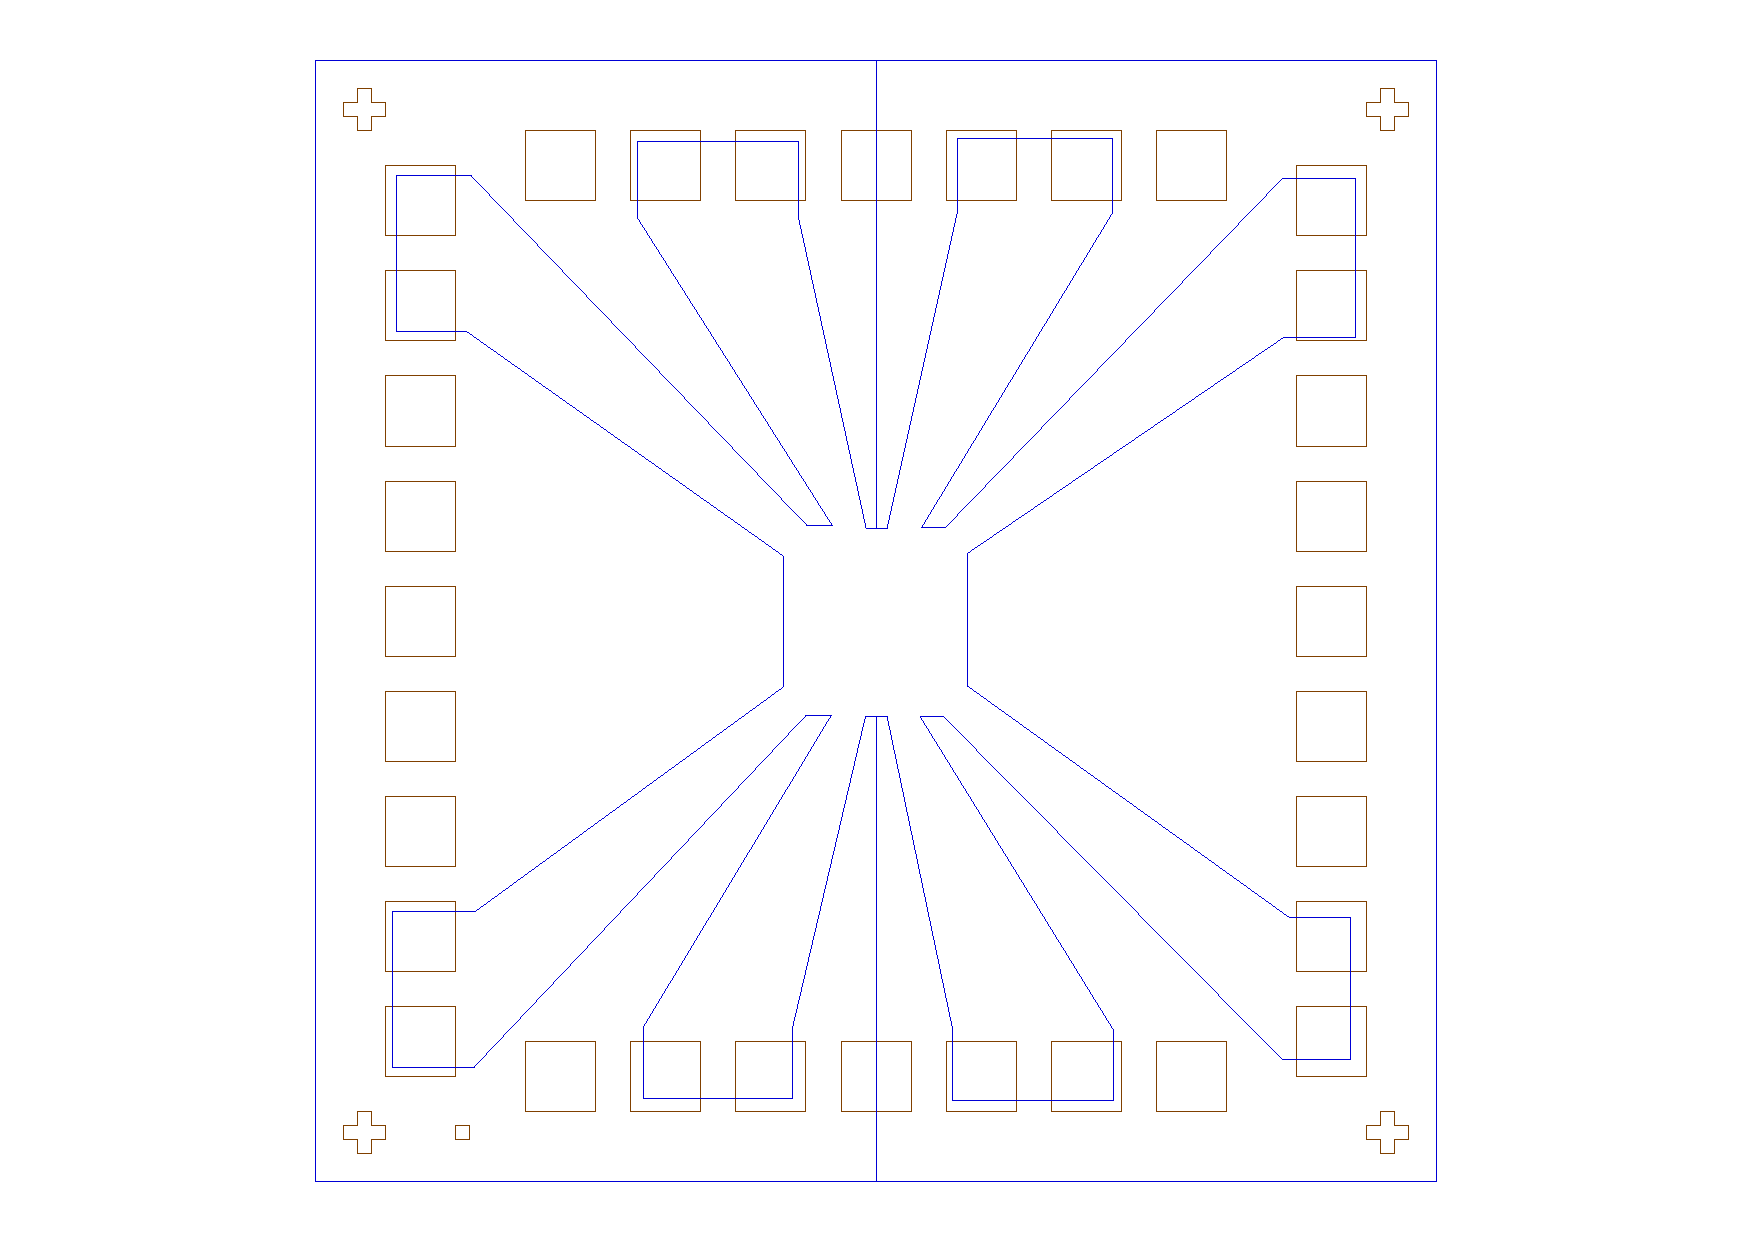
\includegraphics[scale=0.3]{fig/align1.pdf}
\caption{Alignment of the ohmics patern with the mesa patern.} \label{align1}
\end{figure}

\begin{figure} [h] \centering
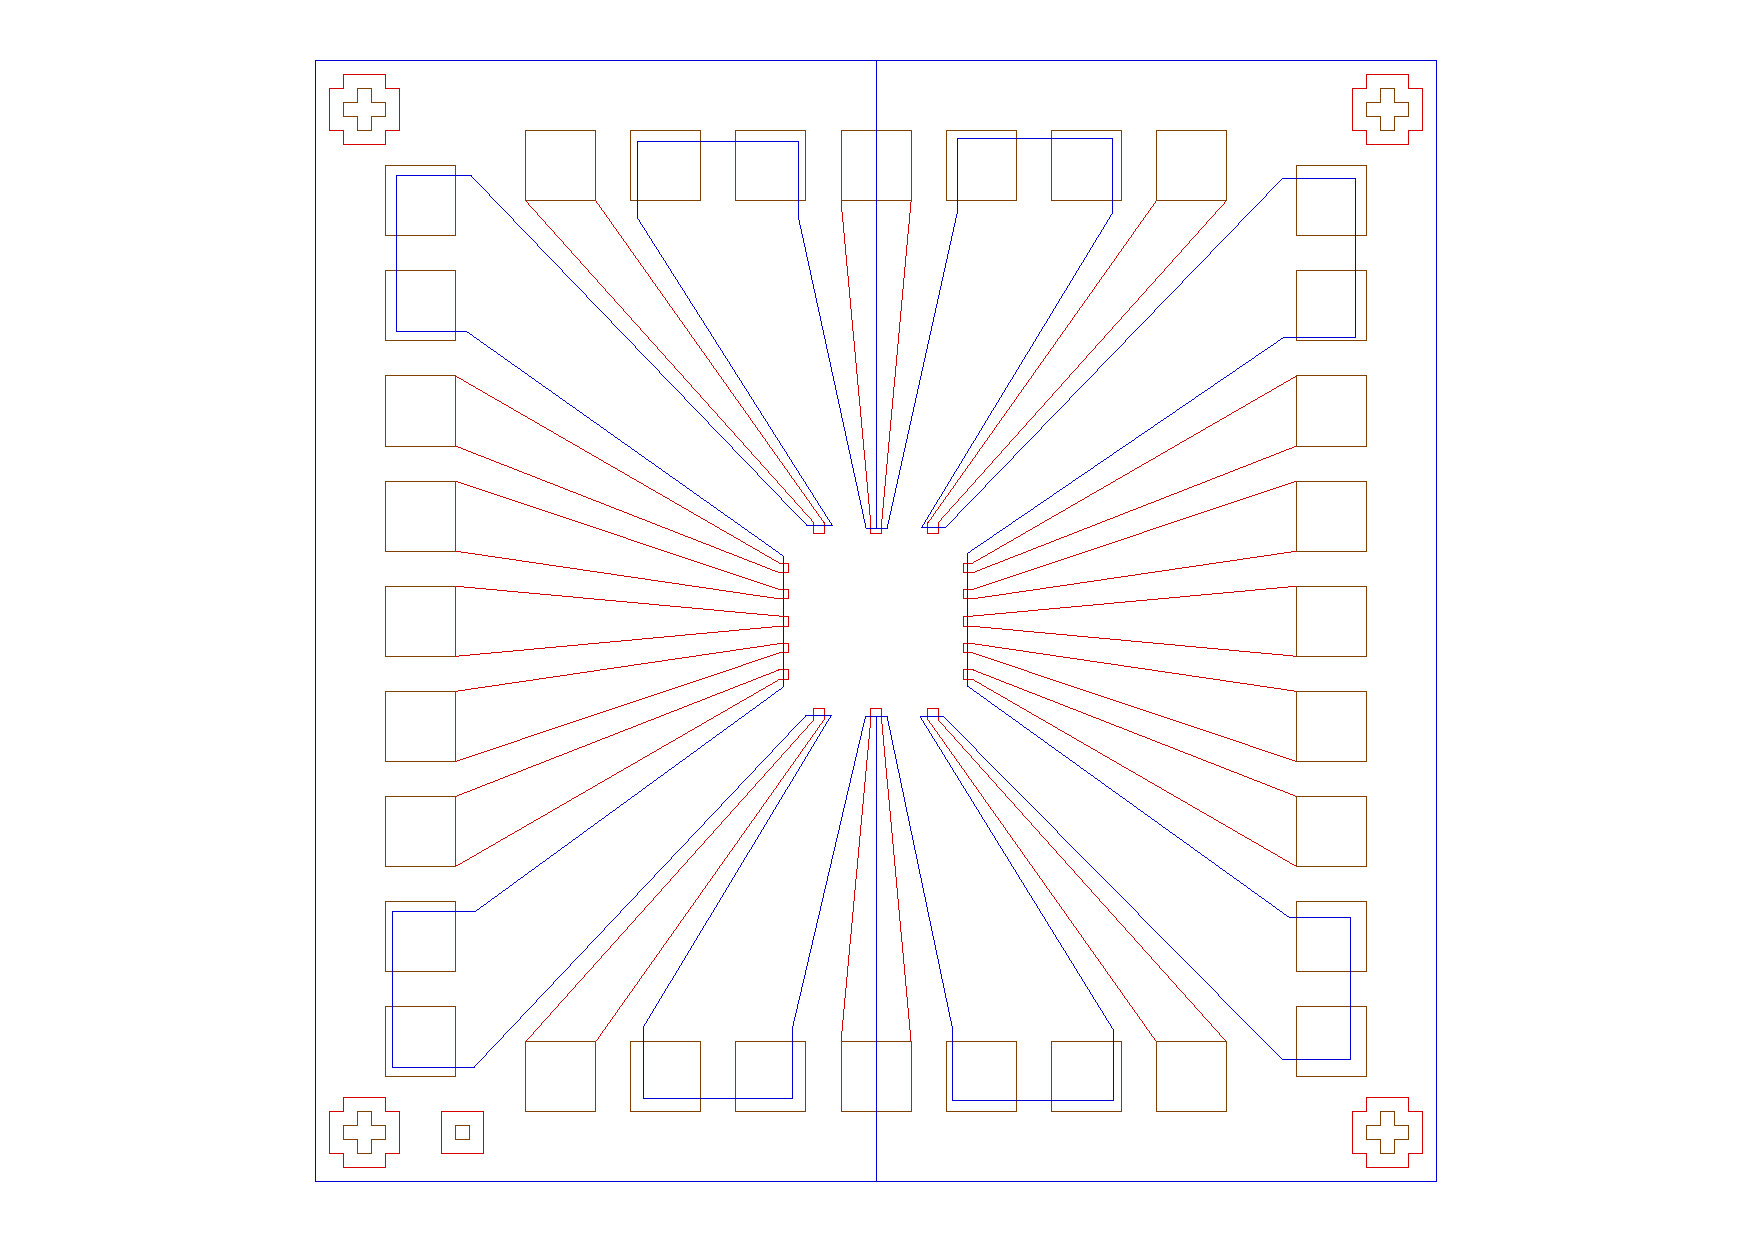
\includegraphics[scale=0.3]{fig/align2.pdf}
\caption{Alignment of the contacts with the ohmics and mesa paterns.} \label{align2}
\end{figure}

\newpage

\subsection{Alignments DD V2}

\begin{figure} [h] \centering
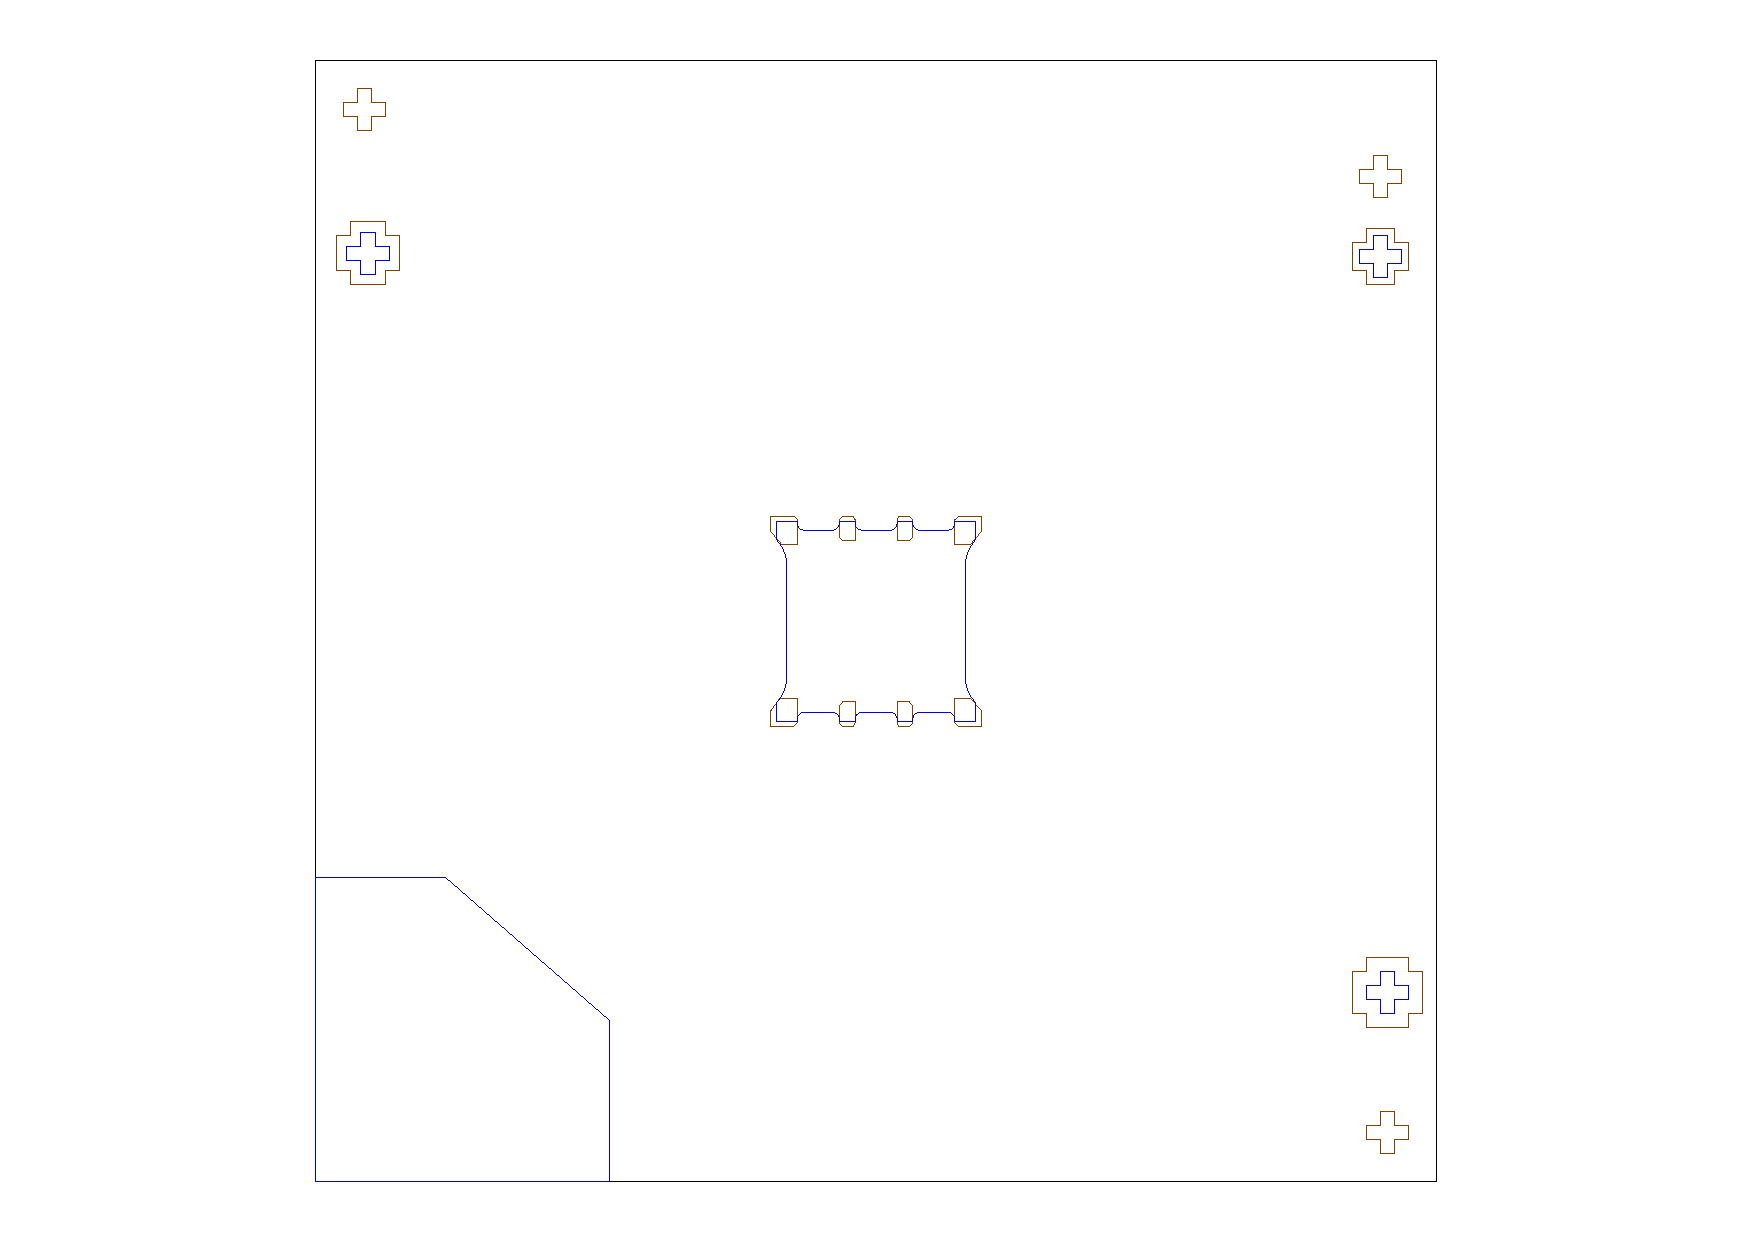
\includegraphics[scale=0.3]{fig/align1_1.pdf}
\caption{Alignment of the ohmics patern with the mesa patern.} \label{align1}
\end{figure}

\begin{figure} [h] \centering
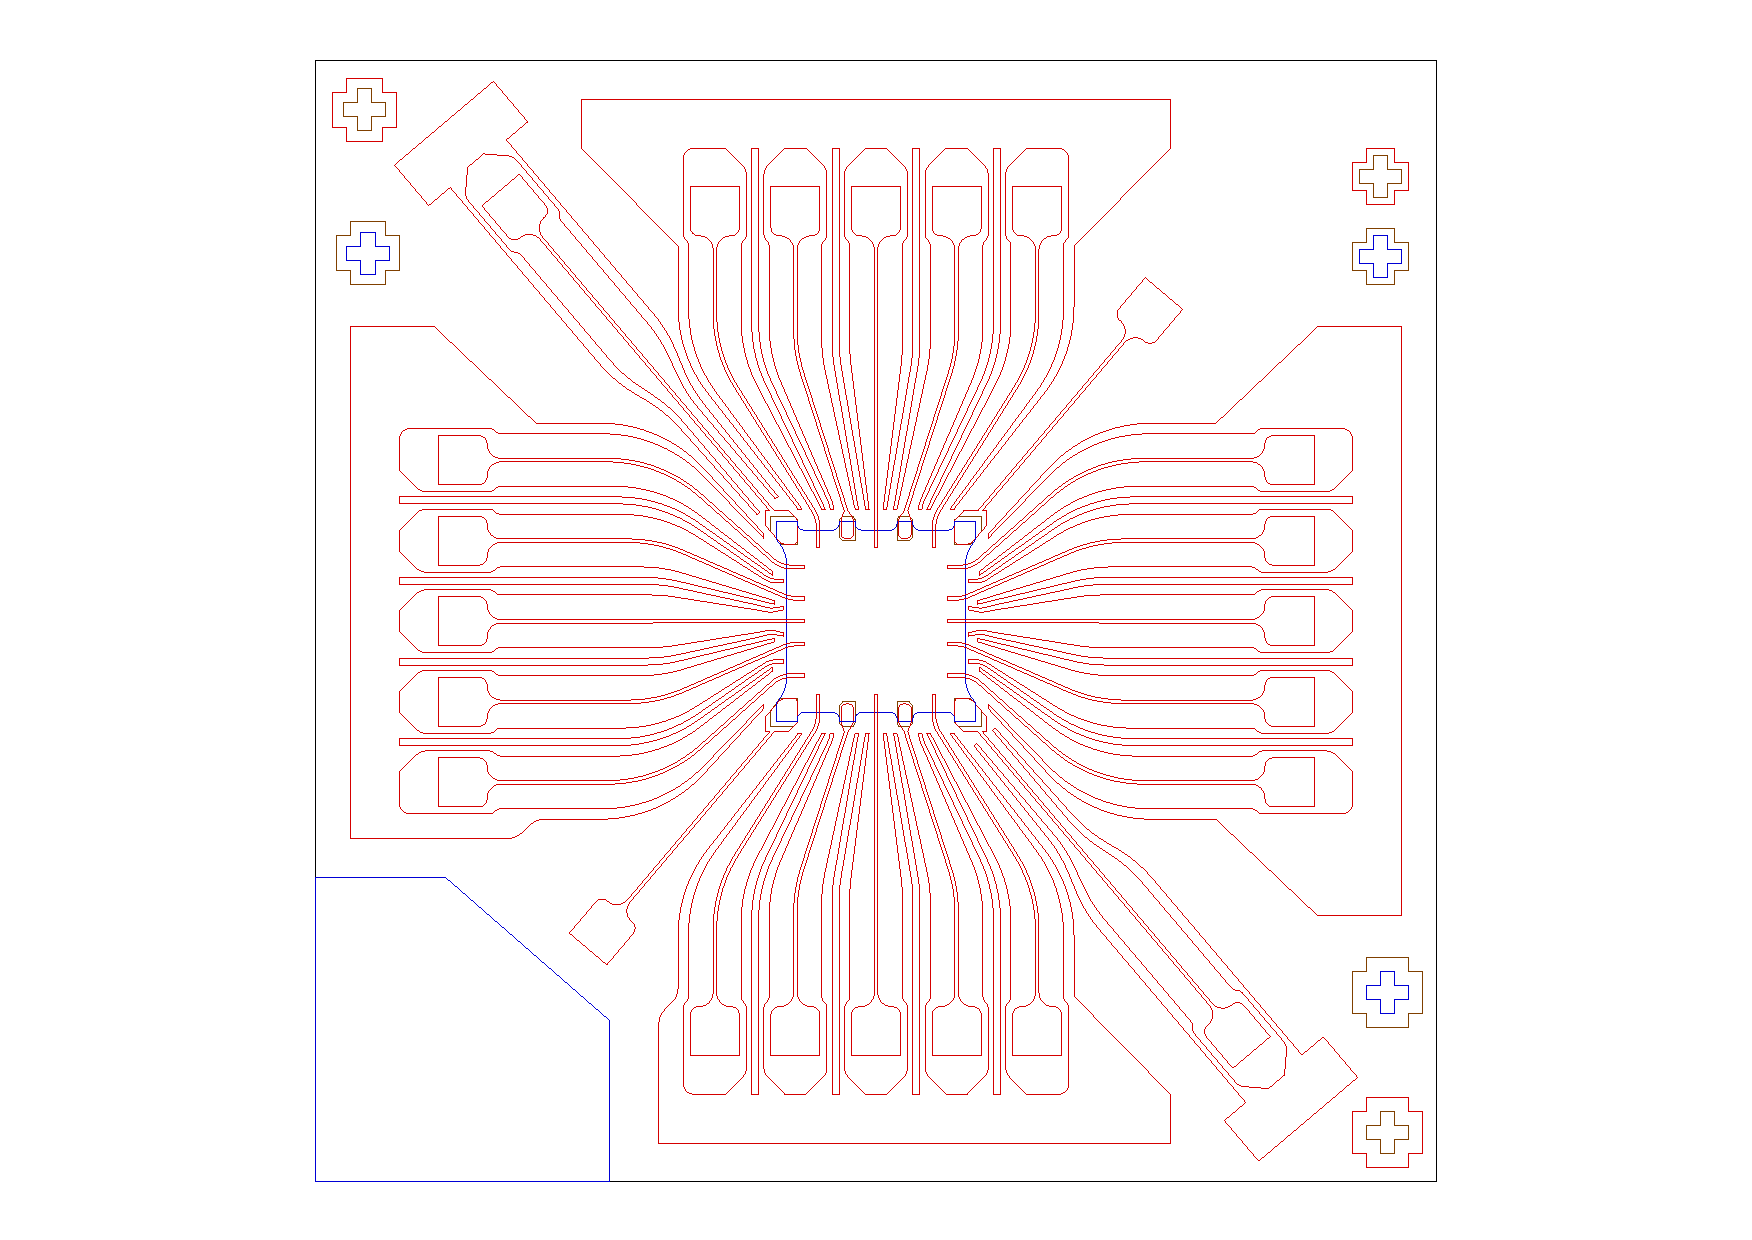
\includegraphics[scale=0.3]{fig/align2_1.pdf}
\caption{Alignment of the contacts with the ohmics and mesa paterns.} \label{align2}
\end{figure}



\newpage

\subsection{Dressing}[noitemsep]
\begin{itemize}
\item mask
\item hair nest
\item suit
\item shoes (!on other side of bench!)
\item gloves
\item glasses
\end{itemize}

The clean room begin just after the bench in front of the door. DON'T SIT ON THE BENCH.

Note: If you have your own cleanroom gown, it can be picked up in the grey area of the Upper East labs.
Tick your name off on the spreadsheet and grab a head cover, overalls and boots from the lockers corresponding
to your size.

\subsection{Misc}

\begin{itemize}
\item Tools in lunch box
\item Clean everything you need/use
\item Write up EVERYTHING, make protocols
\item To quickly remove the water in beakers, spray IPA and blow dry
\item If the chip is flipped: clean and re-spin
\item Inside fume hoods, always manipulate beakers and
chip on wipes (to avoid losing the chip in holes).
\item If a solvent container is empty, open it and let it out gas inside
the cupboard on the left hand side.
\item If the solvent waste is full, take an empty solvent container,
pour the solvent waste in it and put it in the bottom left hand
side shelve, on the left of the cupboard. Put a provided sticker
on it.
\end{itemize}

\newpage

